\section{Runtime}
\label{section:noderuntime}

We define the session runtime in Svr.ts,
named after the endpoint.
It exposes (through the module export) a public API 
(\cref{lst:noderuntimepublicapi})
for the developer to pass in the WebSocket server and application logic
(i.e. their handler implementations).


\begin{itemize}
\item public API -- provide seam for websocket server and implementation
\item private API -- carry out the session
\end{itemize}

\begin{figure}[!h]
\begin{lstlisting}[language=javascript,tabsize=2,title=Svr.ts]
export class Svr {
	constructor(wss: WebSocket.Server,
							initialState: Implementation.S51) { ... }
	...
}
\end{lstlisting}
\captionof{lstlisting}{Public API of Session Runtime for Server Endpoint}
\label{lst:noderuntimepublicapi}
\end{figure}

\subsection{Managing Connections}
\begin{itemize}
\item use set and partial object to keep track of pending connections
\item ws event listeners
\item forward reference that we need to manage cancellations here too
\end{itemize}

\subsection{Executing the EFSM}
\begin{itemize}
\item implementation details delegated to the actual implementation states
\item all non-terminal states will `return' the successor implementation -- very difficult to resolve in the type-checker in the runtime (give example of what it may look like) -- solve by giving each state implementation the `advance' function to respect the event-driven nature of everything, so they can call it on completion
\item visualise the interaction between runtime and states as a sequence diagram for message passing
\item constructor binds all methods (that will be passed to other components0 to `this' because of how javascript works with respect to the scoping of `this' (give short example -- or ignore, if this is in the background for typescript)
\item advance -- use discriminated union to figure out what to pass to the state (send -- sendMessage, receive -- register)
\end{itemize}

\begin{figure}[!ht]
\centering
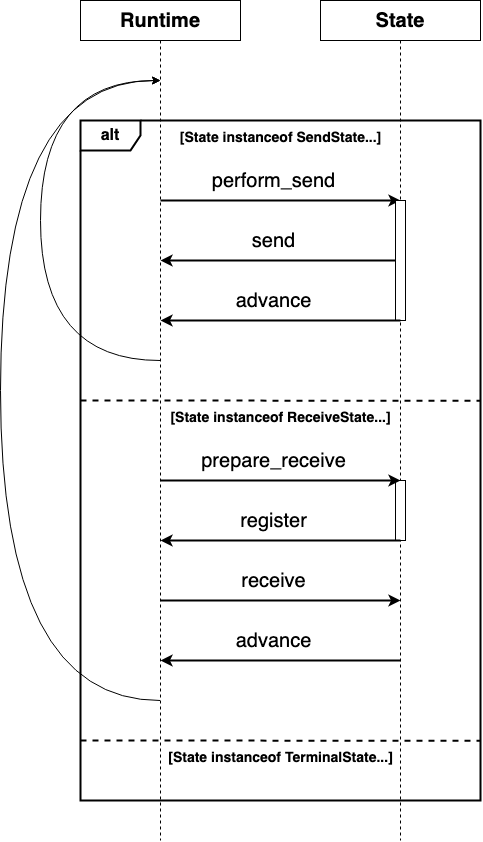
\includegraphics[width=0.5\textwidth]{NodeRuntimeEFSM}
\captionof{figure}{``Message Passing'' Abstraction of EFSM Execution for
Server Endpoints}
\label{fig:noderuntimeefsm}
\end{figure}

\subsection{Handling Message Sends}
\begin{itemize}
\item very short (just for completeness in the report) -- messages are serialised JS objects (in JSON notation) sent and decoded on the other end, type-correct by construction
\end{itemize}

\subsection{Handling Message Receives}
\begin{itemize}
\item motivate the edge case that message can arrive in the websocket (in succession) before the handler is registered
\item motivate the edge case that message can arrive `out of protocol order' 
\item explain the double queue system and how that provides consistency -- emphasising that this works because of the single-threaded typescript runtime
\end{itemize}

\begin{figure}[!ht]
\centering
\begin{subfigure}[b]{0.8\textwidth}
\centering
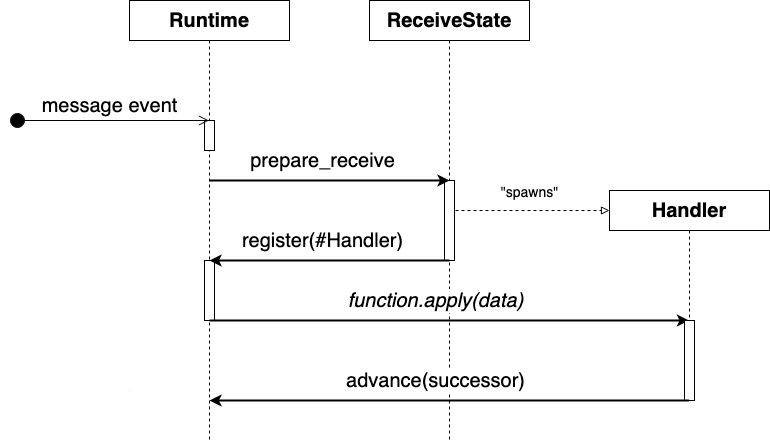
\includegraphics[width=\textwidth]{NodeRuntimeReceive2}
\caption{Message processed before transitioning to receive state}
\label{subfig:nodereceivemsgfirst}
\end{subfigure}
\hfill
\begin{subfigure}[b]{0.8\textwidth}
\centering
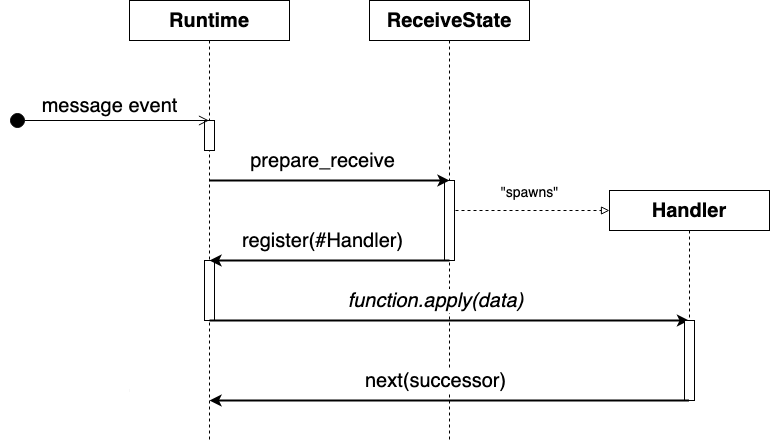
\includegraphics[width=\textwidth]{NodeRuntimeReceive1}
\caption{Message processed after transitioning to receive state}
\label{subfig:nodereceivehandlefirst}
\end{subfigure}
\captionof{figure}{Possible Orderings for Handling Message Event and Preparing
Receive State}
\label{fig:nodereceivecompare}
\end{figure}

\subsection{Handling Termination}
\begin{itemize}
\item design choice that the client is the one that closes the connection because of the centralised role of the server
\item forward reference that this gives opportunity to extend support for general protocols, as in those protocols, the server's terminal state doesn't imply it's terminal for everyone else
\end{itemize}
